\documentclass[a4paper]{article}

%% Language and font encodings
\usepackage[english]{babel}
\usepackage[utf8x]{inputenc}
\usepackage[T1]{fontenc}

%% Sets page size and margins
\usepackage[a4paper,top=3cm,bottom=2cm,left=3cm,right=3cm,marginparwidth=1.75cm]{geometry}

%% Useful packages
\usepackage{amsmath}
\usepackage{graphicx}
\usepackage[colorinlistoftodos]{todonotes}
\usepackage[colorlinks=true, allcolors=blue]{hyperref}

\title{IFT6285 TP}
\author{Jeanne, Jason WU}

\begin{document}
\maketitle

\begin{abstract}
Dans ce travail pratique,  on discutera les methodes de la prédiction d'une séquence de formes à partir d'une séquence de lemmes.
\end{abstract}

\section{Introduction}
Quel sont les lemmas?

En linguistique, les lemmes sont faits de morphèmes. A lemma is the canonical form of a set of words. For example, 'found, finds, find' are forms of the word find as the lemma. As for the words like 'is, are, was, ...' are the forms of the lemma 'be'.

\section{Analyse des données}

\subsection{La relation parmi les train, test et validation données}

We use Training set to train the classifier machine, Then we need to apply our classifier machine on Dev-Test to avoid overfitting situation. But why there is one saying that Naive Bayes classifiers considered relatively immune to overfitting? We still need to find more information.

\begin{center}
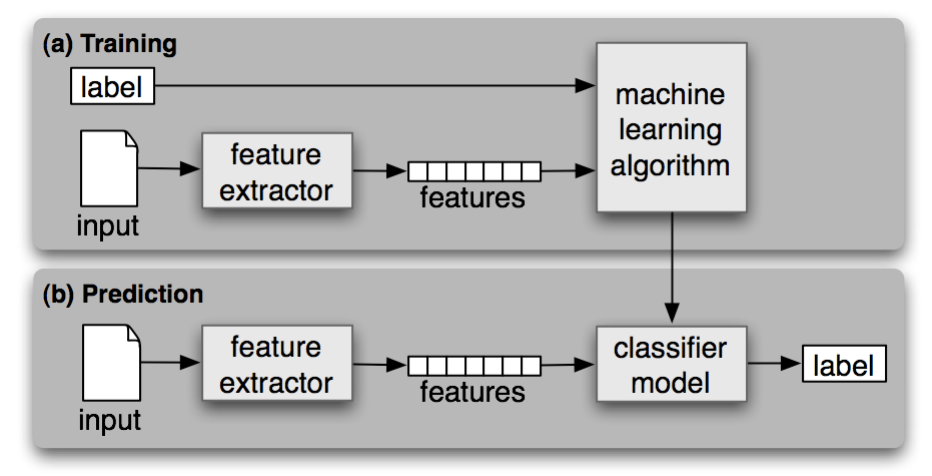
\includegraphics[width=0.8\textwidth]{process_flow.png}
\end{center}

After having our classifier machine, we can use it to predict with input. In our case, that means we can use the classifier model to predict the form for word with the input - lemma. After getting the predicted word, then we can compare with the data in Test set, and get the accuracy for our classifier model/machine.

\begin{center}
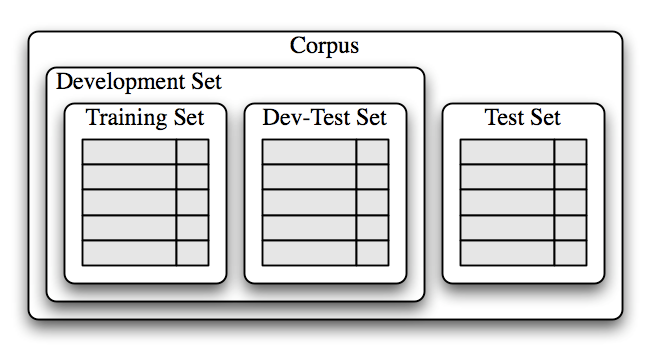
\includegraphics[width=0.8\textwidth]{Corpus.png}
\end{center}

\subsection{La statistique}

\subsection{Réduire les bruits}
Handling the special chacaters, I think it should be some kinds of reduce noise.
\subsection{Baseline}
Si on faisait rien, combien de précision de prédiction a-t-on gagné? 
Less than 0.5 with 1500 sl	ices pairs for training set and 500 pairs for test set.

\section{Outil}
\subsection{Traitement}
\subsubsection{Comparison parmi NLTK, TextBlob, Stanford CoreNLP, SpaCy and Gensim}
\begin{itemize}
\item Modèles entraîné ou pas?
\item La vitesse
\item NLTK vs. spaCy \cite{noauthor_nltk_2016} Selon https://blog.thedataincubator.com/2016/04/nltk-vs-spacy-natural-language-processing-in-python/, spaCy est 20 fois plus vite que NLTK sur le travail de POS.
\end{itemize}
\subsubsection{NLTK}
\begin{enumerate}
\item Il faut considérer que les donnée on va nourrir au NLTK est dans quelle forme. En fait, nous sommes distribué les donnés dans la paire de frome-lemma.
\end{enumerate}

\subsection{Evaluation}
\begin{itemize}
\item Shell
\item Python
\item Excel
\end{itemize}

\section{Fondations de l’Algorithme}
\subsection{N-gram}
Je ne veut pas enlever la ponctuation maintenant. Comme je crois que ils aident la prédiction.  Par example:
- bigram = ('', 'the')       The : the    =  19142.1 : 1.0
Si le mot avant "the" est ""(blank), puis "the" sera "The" avec t en majuscule. Parce que c'est normalement le debut d'une phrase.

\textcolor{red}{Why we consider N-gram? I think for our case, we only use Naive Bayes, not about the N-gram. We extract our feature with bi-words or n-words.}

These words are not independent, if we need to consider all the hypotaxis between these words, we consider to use Markov model to get the probability for the sentence: $P(s)=\prod\limits_{i=1}^{n}P(w_i|w_1...w_{i-1})$

\href{https://en.wikipedia.org/wiki/Markov_chain}{Markov chain}: A Markov chain is "a stochastic model describing a sequence of possible events in which the probability of each event depends only on the state attained in the previous event."

An n-gram model is an expended Markov model, for our case, it means the form for current word, it depends by previous n words. if n = 1, then the form depends by previous word, if n = 2, it's depends by previous 2 words, if n-gram, then we use this one to get the probability for the sentense: $P(s)=\prod\limits_{i=1}^{n}P(w_i|w_{i-n+1},...,w_{i-1})$

n = 1(unigram): $P(s)=\prod\limits_{i}P(w_i)$, e.g. $P(x_1,x_2,...,x_{10}) = P(x_1)P(x_2)...P(x_{10})$

n = 2(bigram): $P(s)=\prod\limits_{i}P(w_i|w_{i-1})$, e.g. $P(x_1,x_2,...,x_{10}) = P(x_1)P(x_2|x_1)P(x_3|x_2)...P(x_{10}|x_9)$

For our case, we predict the sentense, for example: 
s = "Year 208 BC was a year of the pre-Julian Roman calendar." 
That is P(s) = P(Year)P(208|Year)P(BC|208)...P(calendar|Roman)P(.|calendar)

So N-gram helps to predict the sentence.

\subsection{Probabilité Modèle}
\subsubsection{Naïve Bayes}
$ P(A \mid B) = \frac{P(B \mid A) \, P(A)}{P(B)} $

How to predict

\textcolor{red}{How to use smoothing?}
{ Nos variables aléatoires sont discrètes. -> MultiNomial Naive Bayes -> Smoothing}

\textcolor{red}{Is that possible overfit if using Naive Bayes?}

\subsubsection{Modèles de Markov cachée HMM}
\begin{itemize}
\item Théorie
\item Lier les séquences aux états
\item Lissage
\item Apprentissage des paramètres
\end{itemize}


\subsection{Générateur vs Discriminant}

\subsection{Local Maximum}

\subsection{Label bias problem}

\section{Related work}
\section{Discussion}
\section{Résumé}
\cite{greenwade93}


\bibliographystyle{alpha}
\bibliography{bib_jason,sample}
\end{document}